\chapter{Driver de la centrale inertielle (IMU)}

\section{Industrial I/O subsystem}

L’objectif de ce sous-système est de faciliter les interactions utilisateur avec un périphérique depuis l’espace utilisateur d’un système Linux. En général, cela s’adresse aux périphériques réalisant une conversion analogique-numérique ou une conversion numérique-analogique.

\vspace{1cm}

L’accès aux données se fait par l’intermédiaire d’un ou plusieurs fichiers~:

\code{text}
root@raspberrypi0-wifi:~# ls sys/bus/iio/devices/iio\:device0
dev                in_accel_z_raw       in_anglvel_z_raw    power/
in_accel_scale     in_anglvel_scale     in_temp_input       subsystem/
in_accel_x_raw     in_anglvel_x_raw     name                uevent
in_accel_y_raw     in_anglvel_y_raw     of_node/
\end{minted}

Le fichier \codeinline{text}{name} contient le nom du périphérique~:

\code{text}
root@raspberrypi0-wifi:~# cat /sys/bus/iio/devices/iio\:device0/name 
mpu-9250
\end{minted}

\vspace{1cm}

\begin{figure}[H]
    \centering
    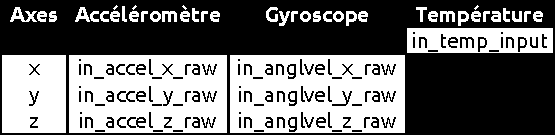
\includegraphics[width=0.5\linewidth]{\figures/tab_imu.pdf}
    \decoRule
    \caption[
    Tableau d'explication des fichiers d'interface du driver de l'IMU]{
    Tableau d'explication des fichiers d'interface du driver de l'IMU}
    \label{fig:Tableau d'explication des fichiers d'interface du driver de l'IMU}
    \end{figure}

\section{Calculs de la position de la centrale inertielle dans l’espace}

Pour l’instant, les calculs sont réalisés avec l’accéléromètre uniquement.

\begin{figure}[H]
    \centering
    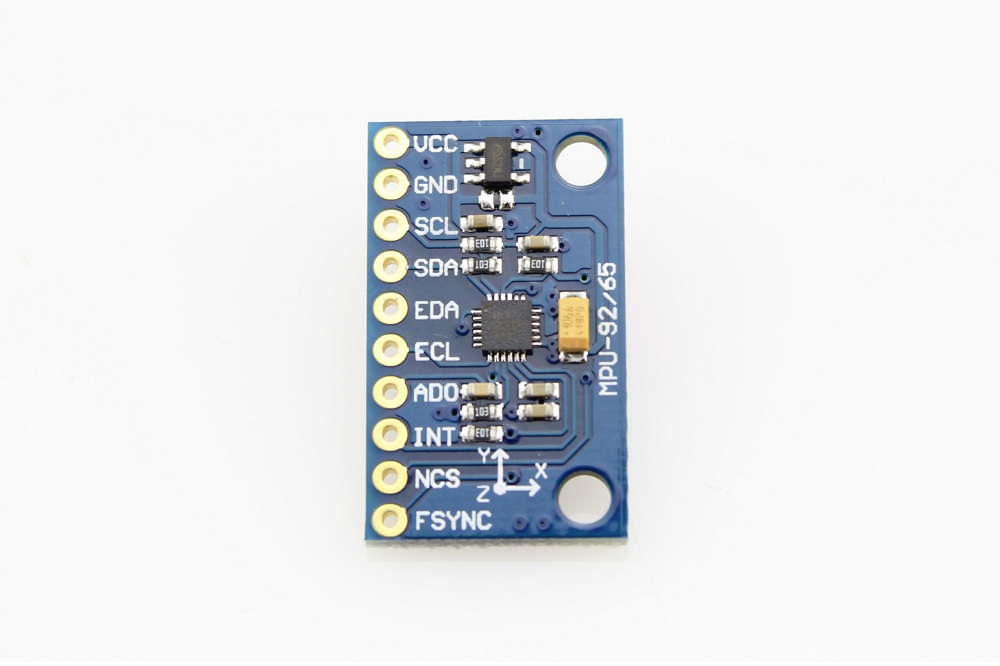
\includegraphics[width=0.5\linewidth]{\figures/photo_imu_test.png}
    \decoRule
    \caption[
    Photo du module IMU utilisé pour les tests]{
    Photo du module IMU utilisé pour les tests}
    \label{fig:Photo du module IMU utilisé pour les tests}
    \end{figure}

\vspace{1cm}

La taille des registres de données de l’accéléromètre est de 16-bits pour chaque axe.

\subsection{Calcul d’angle entre deux vecteurs}

Soit les coordonnées X et Y correspondants aux données de l’accéléromètre.

\vspace{1cm}

Calcul du rayon~:
\begin{align*}
r&=\sqrt{x^{2}+y^{2}}
\end{align*}

%\vspace{1cm}

Calcul de l'angle~:
\begin{align*}
\alpha&=acos\left(\frac{x}{r}\right)\times\frac{180}{\pi}
\end{align*}

\vspace{1cm}

Par exemple, posons $x=512$ et $y=854$~:

\vspace{1cm}

Calcul du rayon~:
\begin{align*}
r&=\sqrt{512^{2}+854^{2}}=995,7
\end{align*}

%\vspace{1cm}

Calcul de l'angle~:
\begin{align*}
\alpha&=acos\left(\frac{x}{r}\right)\times\frac{180}{\pi}=59^{\circ}
\end{align*}

	
